\documentclass{standalone}
\usepackage{tikz}
\usepackage{nono}
\begin{document}
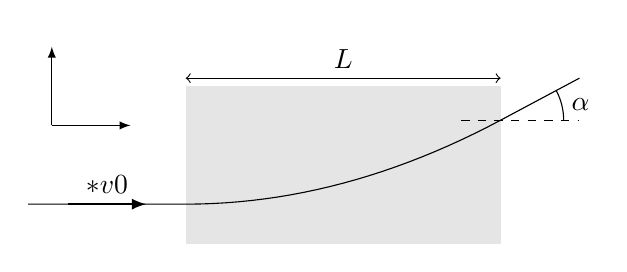
\begin{tikzpicture}
  \fill[gray!20](1, -0.5) rectangle (5, 1.5);
  \draw[<->] (1, 1.6) -- (5, 1.6) node[midway, above]{$L$} ;
  \draw (-1,0) -- (1, 0) plot[domain=1:5](\x,{(\x-1)^2/15}) coordinate(A) -- ++(1, 8/15);
  \draw[-latex, thick] (-0.5, 0) -- (0.5, 0) node[midway, above]{$\vv*{v}{0}$};
  \draw[-latex] (-0.7, 1) -- ++(1, 0) node[right]{$\vex$};
  \draw[-latex] (-0.7, 1) -- ++(0, 1) node[above]{$\vey$};
  \draw[dashed] (A) ++(-0.5, 0) -- ++(1.5, 0);
  \draw (A) ++(0.8, 0) arc(0:{atan(8/15}:0.8) node[midway, right]{$\alpha$}; 
\end{tikzpicture}
\end{document}
